To evaluate the produced \ac{ECD} topologies, topologies are represented as a hypergraph.
Hypergraphs are a generalization of a graph and are formally defined as:
$\mathbf{H} = (\mathbf{V}, \mathbf{E})$, where $\mathbf{V}$ is a set of $N \in \N$ vertices $\{v_1,...,v_N\}$ and $\mathbf{E}$ is a set of $M \in \N$ hyperedges $\{\mathbf{e_1},...,\mathbf{e_M}\}$, where each hyperedge $\mathbf{e_i} \in \mathbf{E}$ is $\mathbf{e_i} \subseteq \mathbf{V}$ \cite{hypergraph_def}.
In matrix notation a hypergraph can be represented in an adjacency matrix \cite{hypergraph_adjacency}.
An example of an adjacency matrix together with the corresponding drawing of a hypergraph can be found in figure \ref{fig:hypergraph_adjacency}.

\begin{figure}
\begin{center}
    % 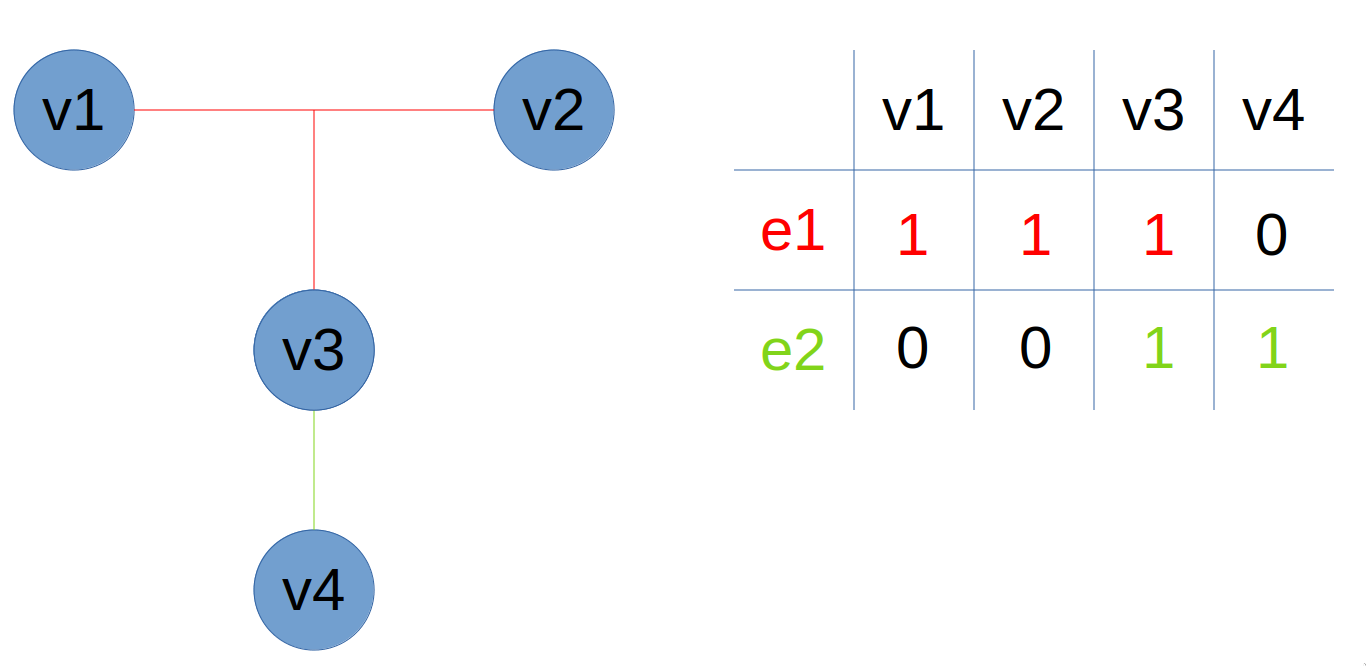
\includegraphics[width=13cm]{imgs/hypergraph_adjacency.png}
    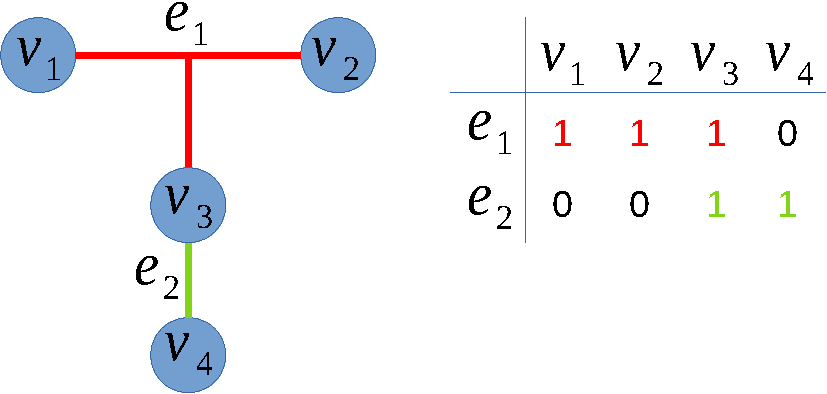
\includegraphics[width=13cm]{imgs/hypergraph_adjacency_cropped.pdf}
    \caption{An example drawing of a hypergraph with its corresponding adjacency matrix. The hypergraph is defined as: $\mathbf{H} = (\mathbf{V}, \mathbf{E})$, $\mathbf{V} = \{v_1, v_2, v_3, v_4\}$, $\mathbf{E} = \{\mathbf{e_1}, \mathbf{e_2}\}$, with $\mathbf{e_1} = \{v_1, v_2, v_3\}$, $\mathbf{e_2} = \{v_3, v_4\}$. In the adjacency matrix a row corresponds to a hyperedge and each column to a vertex. When a vertex is present in a hyperedge it has a 1 as an entry in the matrix, when a vertex is not present it has a 0 \cite{hypergraph_adjacency_my}.}
    \label{fig:hypergraph_adjacency}
\end{center}
\end{figure}
